\documentclass[12pt]{report}

\usepackage{amsmath,amssymb,amsfonts} %In case we need math stuff
\usepackage{graphicx} %For inserting images and stuff
\usepackage{listings} %For inserting code snippets
\usepackage{enumerate} %For fancy enumeration
\usepackage{hyperref}
\usepackage{pdfpages}
\usepackage[margin=2cm]{geometry} %Nice margin setting

\title{ECSE 321 - Intro to Software Engineering\\Design Specification Document - Deliverable 2}
\author{Harley Wiltzer\\Camilo Garcia La Rotta\\Jake Shnaidman\\Robert Attard\\Matthew Lesko}
\date{February 27, 2017}

\begin{document}
\pagenumbering{gobble} %No page number on title page
\maketitle
\newpage
\pagenumbering{arabic} %Arabic numeral page numbers on regular pages
\tableofcontents
\part{Architecture of the Proposed Solution}
\section{Description}
	The software architecture comprises of two different patterns: a Model/View/Controller pattern
	and a Layered Architecture pattern. An "Authentication and Authorization" layer is on top of the
	MVC layer. Once the user is authenticated and authorized, they have access to the MVC layer. The
	MVC system contains three components which interact with each other: 
	\begin{itemize}
		\item Controller
		\item View
		\item Model
	\end{itemize}
	The Model component manages the system data and associated operations on that data; it
	encapsulates all the entities that are part of the model (can be seen in the model class
	diagram). The View component defines and manages how the data is presented to the user. The
	Controller component manages user interaction (key presses, mouse clicks, etc.) and passes these
	interactions to the View and the Model.
\section{Rationale}
	The MVC pattern was chosen because this allows the components to be changed independently. For
	example, adding a new view or changing an existing view can be done without any changes to the
	underlying data in the model. It allows the data to change independently of its representation
	and vice versa. Moreover, it supports presentation of the same data in different ways with changes made in
	one representation shown in all of them. \\
	Furthermore, the Model-View-Controller pattern makes multiplatform development very convenient.
	Using this paradigm, equivalent code may be generated for the model component on all platforms,
	as the model is isolated from the other components. Then, the views are isolated from the
	controllers so that modifications to the view classes do not affect code for other platforms
	that utilize the controller classes.\\
	The Layered Architecture pattern was used because the user would need to first authenticate
	him/herself and then receive authorization in order to interact with the sublayer.
\section{Block Diagram}
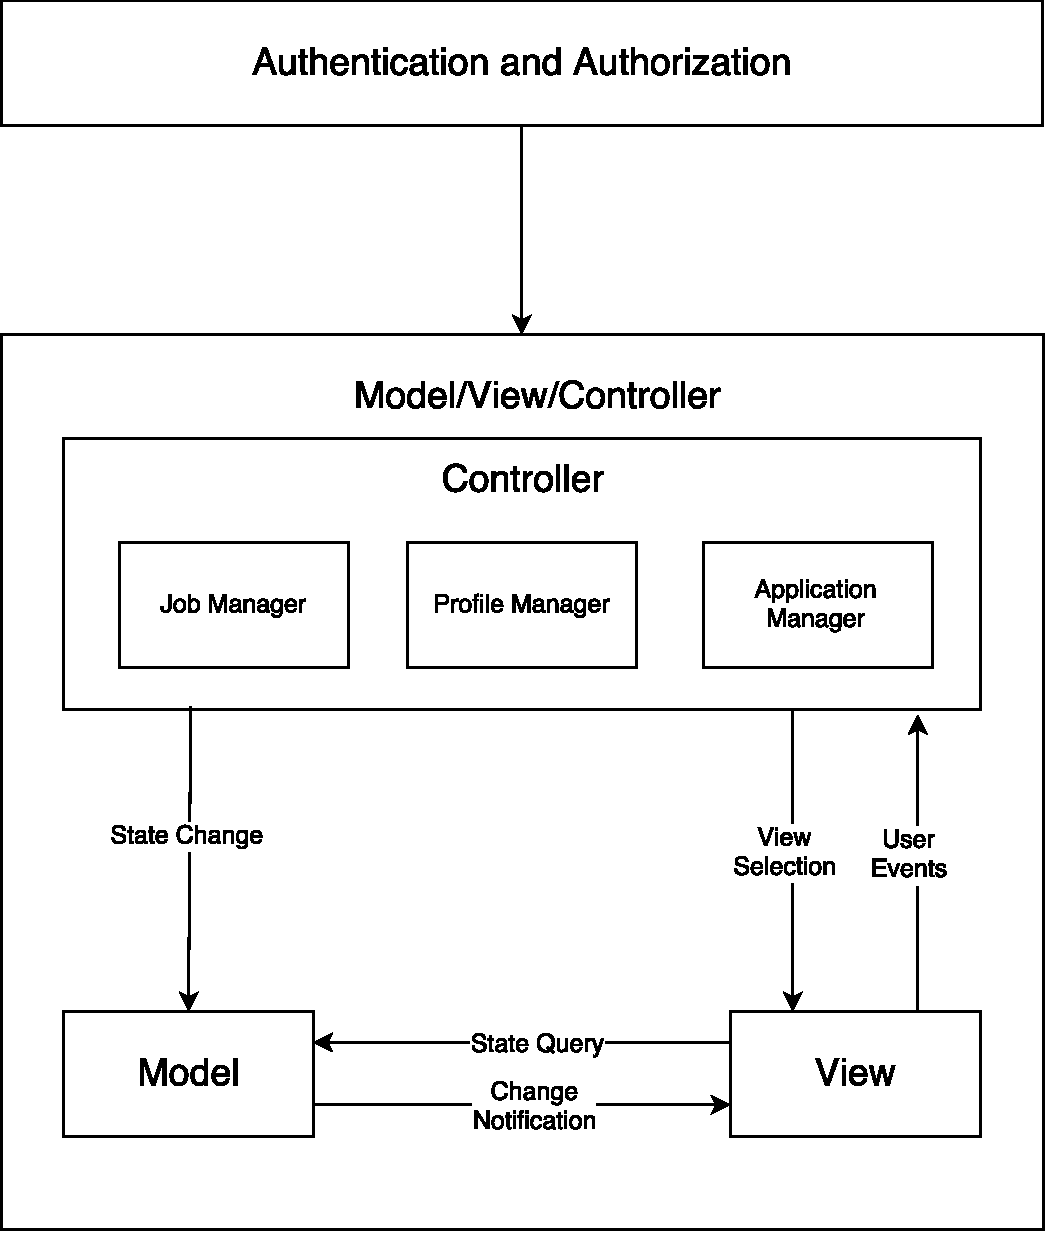
\includepdf[scale=0.5,pages=1]{Architecture/blockDiagram}

\part{Description of the Detailed Design}
\section{Description}
\subsection{Detailed Domain Model}
The Detail Design Diagram consists of the following entities: ApplicationManager, ProfileManager,
CourseManager, Application, Profile, Course, Job, Instructor, Admin, Student, Laboratory, and
Tutorial. It consists of a Controller, called Controller, a Boundary, called View, and a
Persistence, called Persistence XStream. The Controller uses the entities ApplicationManager,
ProfileManager, and CourseManager to save, edit, and modify data within the model, which are then
saved within a persistence layer. The functionalities of the three "Manager" classes are listed
below.
\begin{itemize}
	\item The ApplicationManager is in charge of Applications, which represent the job application
		created and submitted
		by the student for a job. Furthermore, the ApplicationManager is also in charge of managing
		Job data. It is associated with Application, Job, and ProfileManager.
	\item ProfileManager creates and manages Admin, Instructor, and Student entities, all of which inherit from
		the Profile class.
	\item CourseManager creates and manages Course entities.
\end{itemize}
\subsection{Controller Classes}
In total there will be three controller classes in the Controller Packages with an additional class
for input exceptions or input validation. Each controller class has an associated Manager class, and
is in charge of utilizing the manager class safely so that appropriate data is guaranteed to be
entered into the persistence layer.\\
The Controller classes serve the purpose of isolating the model from the input, keeping in mind the
philosophies of the Model-View-Controller paradigm.
\subsection{View Classes}
Finally, there are multiple View classes, dependent on the application platform, that act as
boundary classes. These classes are in charge of gathering user input in a user-friendly manner. The
Web and Mobile applications have four and two Views, respectively, and the Desktop application has
five Views.\\
The View classes are listed by platform below:
\subsubsection{Current Desktop Views}
\begin{enumerate}
	\item \texttt{MenuView}: Allows user to select which functionality to perform
	\item \texttt{RegisterView}: Allows user to enter profile information to create a
		\texttt{Student}, \texttt{Instructor}, or \texttt{Administrator}
	\item \texttt{CreateCourseView}: Allows user to enter data to create a \texttt{Course} given a specific
		\texttt{Instructor}
	\item \texttt{PublishJobView}: Allows user to enter information required for creating a
		\texttt{Job}
	\item \texttt{ApplicationView}: Allows user to create an \texttt{Application}
\end{enumerate}
\subsubsection{Current Mobile Views}
\begin{enumerate}
	\item \texttt{MainActivity}: Allows user to select which functionality to perform (analogous to
		\texttt{MenuView})
	\item \texttt{ApplyToJob}: Allows user to create an \texttt{Application} (analogous to
		\texttt{ApplicationView})
\end{enumerate}
\subsubsection{Current Web Views}
\begin{enumerate}
	\item \texttt{index}: Allows user to select which functionality to perform (analogous to
		\texttt{MenuView})
	\item \texttt{createCourse}: Allows user to enter data to create a \texttt{Course} (analogous to
		\texttt{CreateCourseView})
	\item \texttt{createInstructor}: Allows user to enter data to create an \texttt{Instructor}
		(analogous to \texttt{RegisterView}). This View is temporary and will only be used for this
		Deliverable, as it does not satisfy the requirements of the project.
	\item \texttt{job}: Allows user to submit data to publish a \texttt{Job} (analogous to
		\texttt{PublishJobView})
\end{enumerate}
\section{Rationale}
The program was designed this way so as to follow the principles of the Model-View-Controller design
pattern. As discussed previously, this allowed for the effective isolation of the user input and the
domain model. The Controller classes, along with the \texttt{PersistenceXStream} class, allow for
persistence to be carried out in a safe manner. The Controller classes are designed in such a way
that by using them to create their associated objects, the created objects will automatically be
stored within the persistence layer assuming they were created successfully. To avoid storing faulty
objects, the \texttt{InputException}, as well as several validation classes in PHP, were created. As
such, the Controller classes throw exceptions when unworthy data is passed. The ultimate benefit to
using this design is that the persistence is taken care of at the level of the controller classes,
so the programmer needn't worry about it when designing the Views. With this foundation, the model
may be altered reliably.\\\\
By perusing the list of Views, it is clear that the mobile and web Views are very similar to the
desktop Views in terms of their purposes. This was done to create consistent interfaces across the
platforms. The desktop has many views because it is meant to be used by Administrators, who can
implement the functionalities possible on all other platforms.

%\subsection{Detailed Domain Model}
%The three Manager classes were needed in order to give functionality to the user to create the
%entities associated with the manager classes, except for ApplicationManager creating a
%ProfileManager. The reason ApplicationManager is associated to ProfileManager is because otherwise
%the only way for ApplicationManager to have access to Student is by a direct association to it; this
%would cause a redundancy as now two manager classes are able to create Student entities, which is
%something we want to avoid. Having a separate controller for each manager class allows one to modify
%the functionality of one controller class with its respective manager class without it having to
%affect the other controller classes.
\end{document}
